\subsubsection*{The Codegenerator Visitor}
When the code generator is called from the \texttt{main()} class, the \acrshort{ast} is used to accept a \texttt{CodeGeneratorVisitor} as seen on \myref{fig:CodeGeneratorVisitor}.

\begin{figure}[!ht]
\centering
 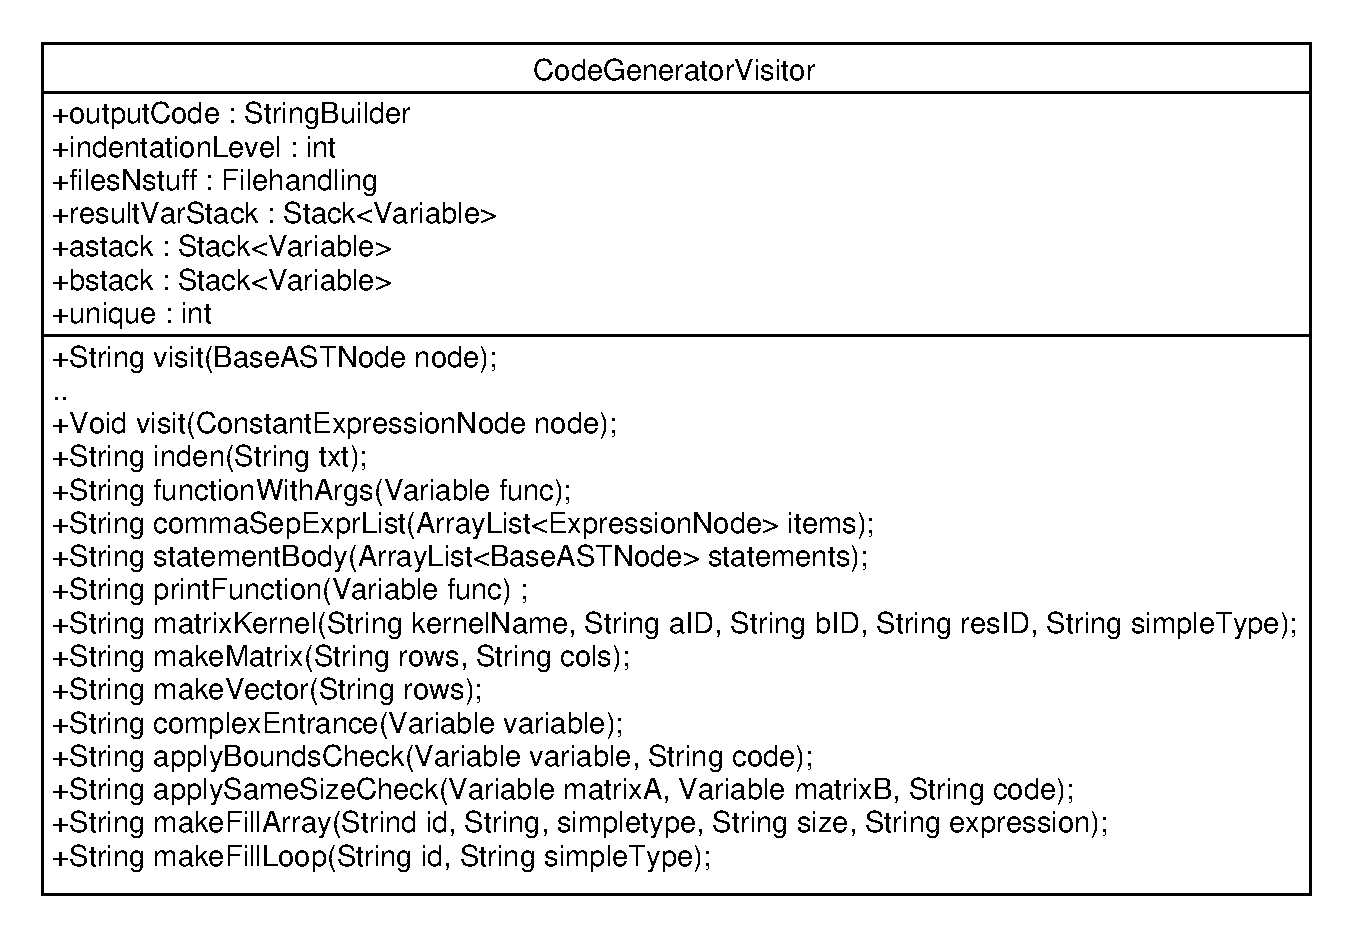
\includegraphics[width=0.60\textwidth]{figures/ClassDiagrams/CodeGeneratorCall.pdf} % trim=4.85cm 15cm 0.85cm 1cm
\caption{A diagram showing the call from the code generator to the visitor which makes the string from the decorated \acrshort{ast}.}\label{fig:CodeGeneratorVisitor}
\vspace{-15pt}
\end{figure}

The visitor builds a string by traversing the nodes of the tree.
Some visit methods like a visit method for a \texttt{ConstantExpressionNode} returns a string.
This string is then used as an argument in other visit methods e.g. \texttt{AssignmentNode} which then produces a string which is a statement that can be executed in C.
This string from \texttt{AssignmentNode} is then appended to the string, containg the object code created by the \gls{gamble} compiler when all the nodes from the decorated \acrshort{ast} have been visited.
%%%%%%%%%%%%%%%%%%%%%%%%%%%%%%%%%%%%%%%%%%%%%%%%%%%%%%%%%%%%%%%%%%%%%%%%%%%%%%%%%%%%%%%%%%%%%%%%%%

As a result the information bubbles upwards from the leafs of the tree to the statementnodes.
The information is put in the correct statementnodes because the visitor pattern makes it possible to specify the route of traversal.
The \texttt{CodeGeneratorVisitor} also contains other methods for producing certain C constructions using the similar \gls{gamble} constructions found in the \acrshort{ast}.
These methods can also be seen on \myref{fig:CodeGeneratorVisitor}.
Some of these methods also make runtime checks of matrices, as matrices needs to be of compatible sizes for some of the operations which can be performed on a matrix, furthermore an index check is implemented such that an out of bounds error will occur if one tries to access memory beyond the bounds of the matrix.
When multiplying two matrices the left matrix of the multiplication has to be a $ N \times M $ while the right one has to be a $ M \times P $ matrix.
So the right matrix must have the same number of columns as the right matrix has rows.
If performing a matrix index multiplication, where every index is multiplied with the corresponding index of the the other matrix, the matrices have to have the same number of rows and columns.

These checks will be inserted as a surrounding if statement around the matrix calculations, so they have to pass these checks before the calculation will be done.
The reason this is done at run-time instead of compile-time is because the sizes of matrices can be dynamic, which results in making it impossible to check for this at compile-time.

When the string is complete it is printed into a file called code.c, along with all the other files needed for running the code, e.g. the kernels used for performing computations on the \acrshort{gpu}.
The code.c file is structured so that it is a valid C program.
First off are the libraries included that C uses, then follows a list of prototypes which are all the \gls{gamble} functions translated into C code, both the user made and libraries.
After the prototypes the main function is made which consists of all the statements in the \gls{gamble} sourcecode translated into C.
After the main method all the implementations of the prototypes are made.